\ifx\wholebook\relax \else
\documentclass[b5paper]{ctexart}
\usepackage[nomarginpar
  %, margin=.5in
]{geometry}

\addtolength{\oddsidemargin}{-0.05in}
\addtolength{\evensidemargin}{-0.05in}
\addtolength{\textwidth}{0.1in}
\usepackage[cn]{../../../prelude}

\setcounter{page}{1}

\begin{document}

\title{二项式堆、斐波那契堆、配对堆}

\author{刘新宇
\thanks{{\bfseries 刘新宇 } \newline
  Email: liuxinyu95@gmail.com \newline}
  }

\maketitle
\fi

\markboth{二项式堆、斐波那契堆、配对堆}{基本算法}

\ifx\wholebook\relax
\chapter{二项式堆,斐波那契堆、配对堆}
\numberwithin{Exercise}{chapter}
\fi

\section{简介}
\label{introduction}

二叉堆使用二叉树存储元素,将二叉树扩展成$k$叉树\cite{K-ary-tree}($k>2$)甚至多棵树可得到更丰富的堆结构。本章介绍二项式堆,它由多棵$k$叉树的森林组成。如果延迟执行二项式堆的某些操作,就可以得到斐波那契堆。斐波那契堆将堆合并的性能从对数时间复杂度提升到常数时间,这对于图算法很重要。本章还介绍配对堆。它在实际中拥有最好的性能。

\section{二项式堆}
\label{sec:binomial-heap} \index{二项式堆}

二项式堆得名于牛顿二项式。它由一组$k$叉树的森林组成,每棵树的大小为二项式展开中的各项系数。牛顿证明了形如$(a + b)^n$的二项式展开后,各项系数可以表示为:

\be
(a + b)^n = a^n + \binom{n}{1} a^{n-1}b + ... + \binom{n}{n-1} a b^{n-1} + b
\ee

当$n$为自然数时,各项系数就呈现出帕斯卡三角形中的一行,如下图所示\footnote{中国称“贾宪”三角形。贾宪(1010-1070),牛顿在1665年证明了$n$为有理数时的情形,欧拉后来将$n$推广到实数。}\cite{wiki-pascal-triangle}。

\begin{verbatim}
    1
   1 1
  1 2 1
 1 3 3 1
1 4 6 4 1
...
\end{verbatim}

有多种方法可以产生一系列二项式系数,其中一种是使用递归。帕斯卡三角形中第一行为1,任何一行的两端为1,其它数字是上一行中左上和右上数字之和。

\subsection{二项式树}
\label{Binomial tree} \index{二项式树}

一棵二项式树是一棵多叉树,并带有一个整数的秩(rank)。记秩为0的二项式树为$B_0$,秩为$n$的二项式树为$B_n$。

\begin{enumerate}
\item $B_0$树只包含一个节点;
\item $B_n$树由两棵$B_{n-1}$树组成,其中根节点元素较大的一棵是另一棵最左侧的子树。如图\cref{fig:link-bitree}所示。
\end{enumerate}

\begin{figure}[htbp]
  \centering
  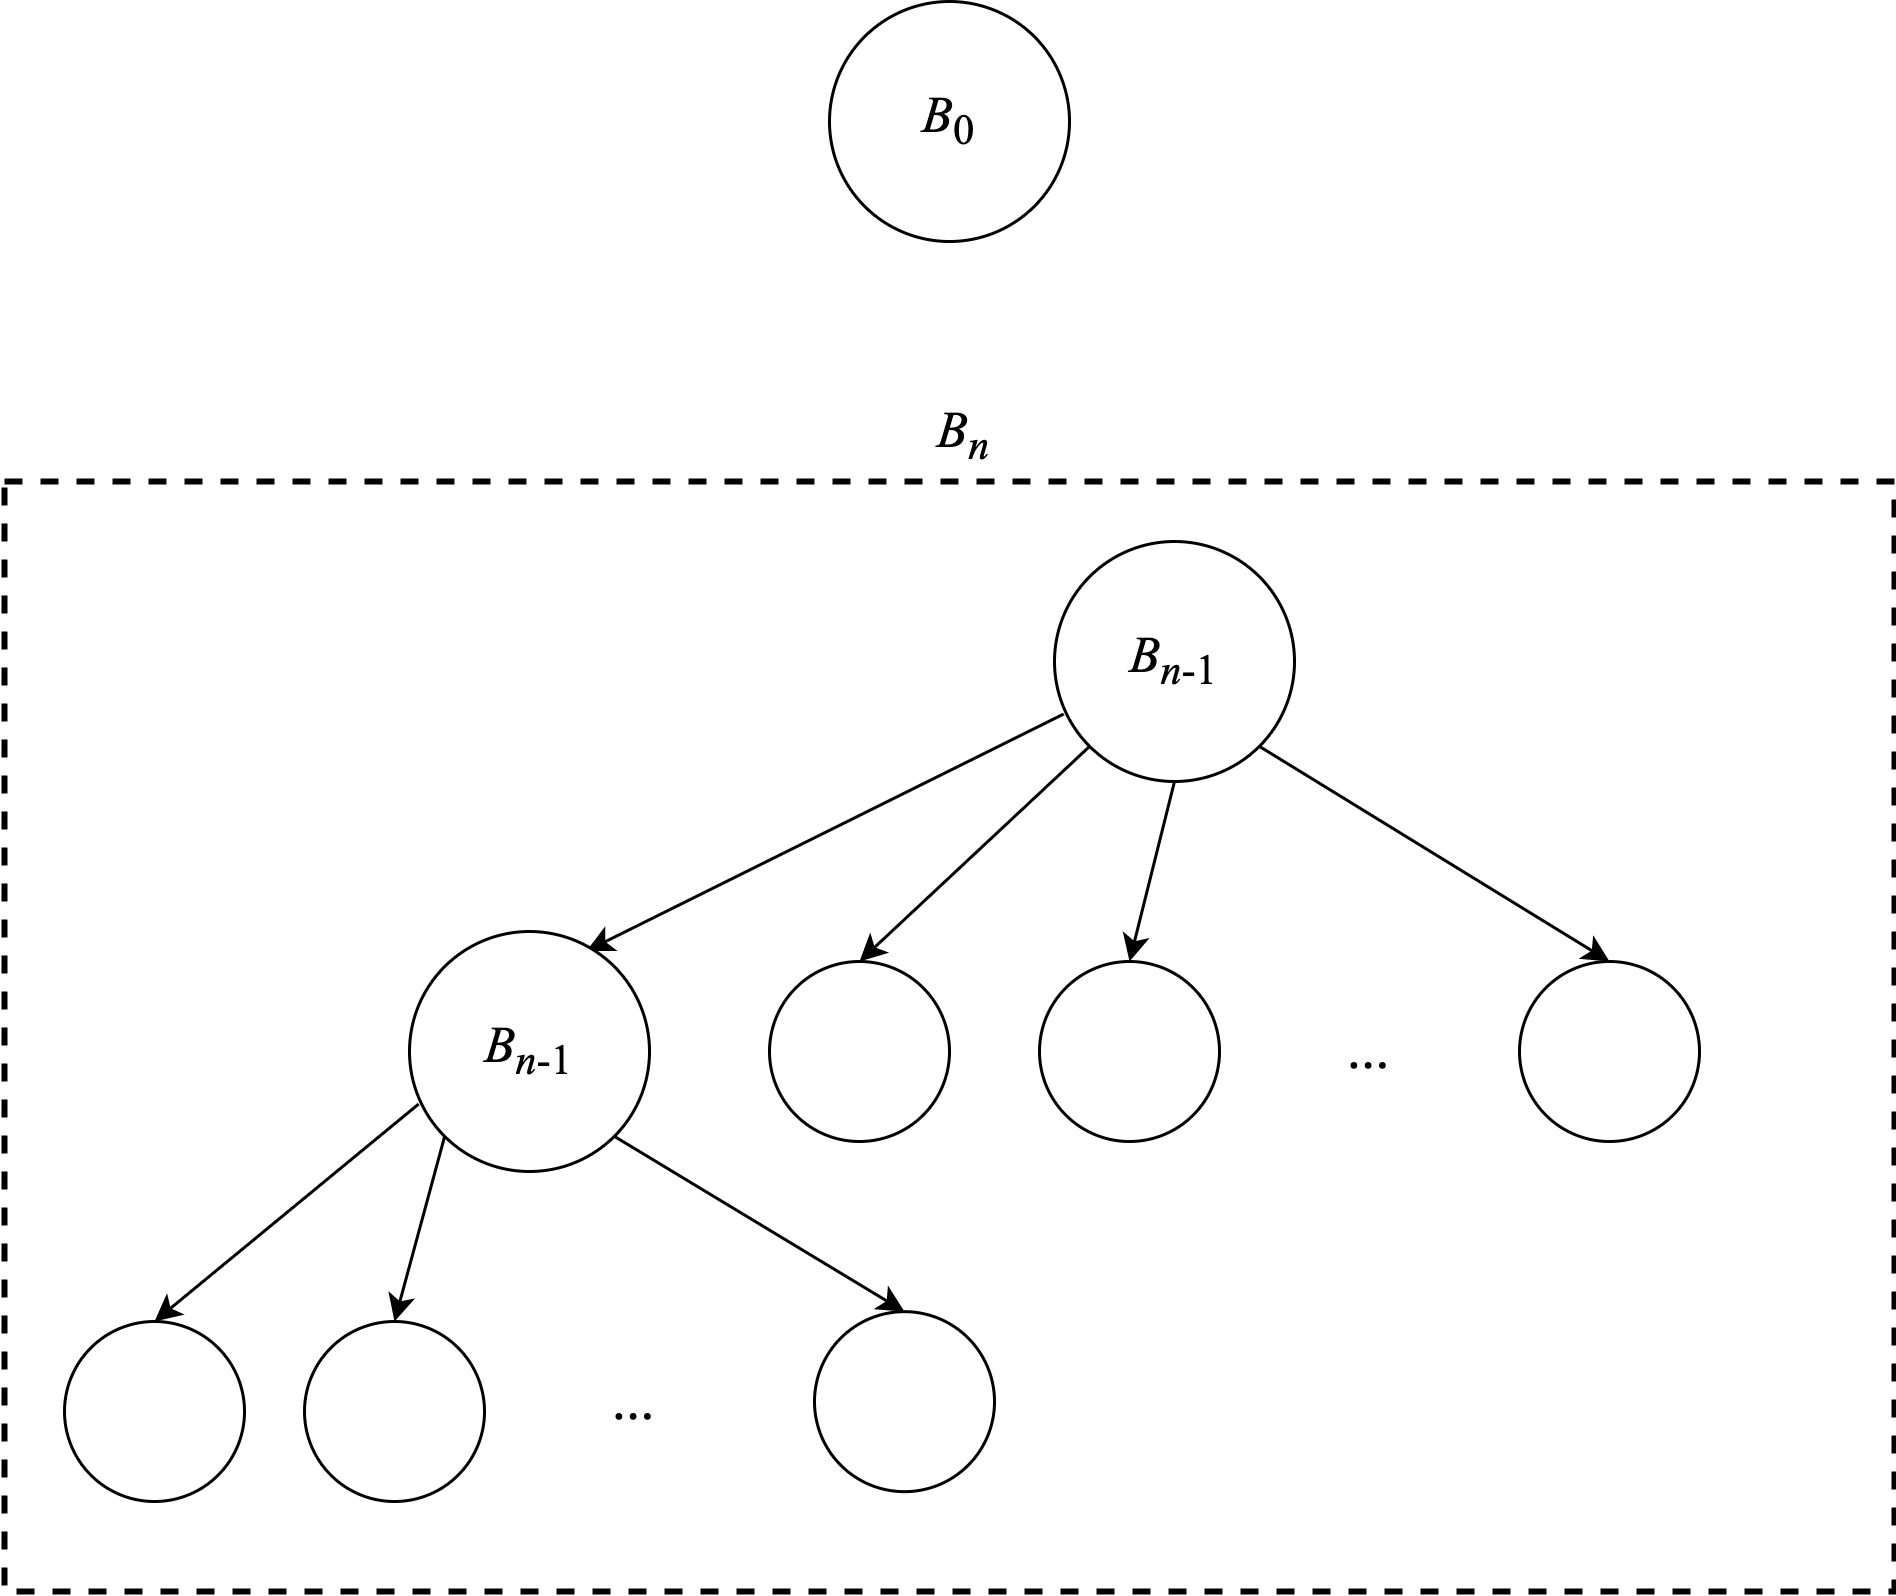
\includegraphics[scale=0.5]{img/btrees}
  \caption{二项式树}
  \label{fig:link-bitree}
\end{figure}

图\cref{fig:bitree-forms}给出了秩为0到4的二项式树例子:

\begin{figure}[htbp]
  \centering
  \subcaptionbox{$B_0$}{\hspace{0.05\textwidth}\includegraphics[scale=0.5]{img/b0tree}\hspace{0.05\textwidth}}
  \subcaptionbox{$B_1$}{\hspace{0.05\textwidth}\includegraphics[scale=0.5]{img/b1tree}\hspace{0.05\textwidth}}
  \subcaptionbox{$B_2$}{\includegraphics[scale=0.5]{img/b2tree}}
  \subcaptionbox{$B_3$}{\includegraphics[scale=0.5]{img/b3tree}} \\
  \subcaptionbox{$B_4$}{\includegraphics[scale=0.5]{img/b4tree}……}
  \caption{秩为0、1、2、3、4……的二项式树}
  \label{fig:bitree-forms}
\end{figure}

观察这些二项式树,可以发现$B_n$中每行的节点数目恰好是二项式系数。例如$B_4$第0层有1个节点(根节点),第1层有4个节点,第2层有6个节点,第3层有4个节点,第4层有1个节点。它们恰好是帕斯卡三角形的第4行(从第0行开始):1、4、6、4、1。这就是二项式树名字的由来。进一步我们可以得知二项式树$B_n$中含有$2^n$个元素。

\index{二项式堆!定义}
一个二项式堆包含一组二项式树(二项式树森林),它满足如下性质:

\begin{enumerate}
\item 每棵树都满足\textbf{堆性质},对于小顶堆,任意节点元素都不小于($\geq$)父节点元素;
\item 堆中任何两棵二项式树的秩都不同。
\end{enumerate}

从性质2可以导出一个结果:含有$n$个元素的二项式堆,如果将$n$转换为二进制数$(a_m ... a_1 a_0)_2$,其中$a_0$是最低位(LSB),$a_m$是最高位(MSB),若$a_i=0$,则堆中不存在秩为$i$的二项式树,若$a_i = 1$,则堆中一定含有一棵秩为$i$的树。例如,设二项式堆含有5个元素,5的二进制为101,堆中含有两棵二项式树,一棵秩为0、一棵秩为2。图\cref{fig:bheap2}中的二项式堆含有19个元素,$19 = (10011)_2$,含有一棵$B_0$树、一棵$B_1$树、一棵$B_4$树。

\begin{figure}[htbp]
  \centering
  \includegraphics[scale=0.5]{img/bheap2}
  \caption{含有19个元素的二项式堆}
  \label{fig:bheap2}
\end{figure}

我们将二项式树定义为多叉树,带有一个根节点元素$k$、秩$r$、和若干子树$ts$,记为$(r, k, ts)$。定义二项式堆为按照秩递增的二项式树的列表:

\lstset{frame=single}
\begin{Haskell}
data BiTree a = Node Int a [BiTree a]

type BiHeap a = [BiTree a]
\end{Haskell}

\index{左侧孩子,右侧兄弟}
有一种叫做“左侧孩子,右侧兄弟”\cite{CLRS}的方法,可以复用二叉树的结构来定义多叉树。每个节点包含左侧和右侧部分:左侧部分指向节点的第一棵子树,右侧部分指向兄弟节点。所有兄弟节点组成一个链表,如图\cref{fig:lcrs}所示。也可以直接利用数组或列表来表示一个节点的子树。

\begin{figure}[htbp]
  \centering
  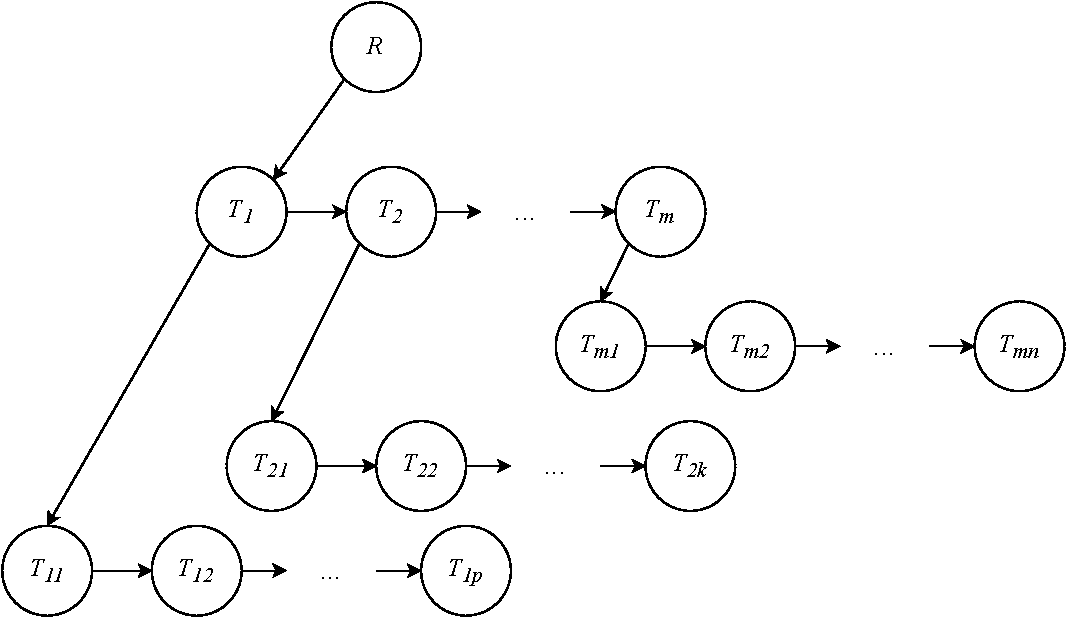
\includegraphics[scale=0.5]{img/left-child-right-sibling}
  \caption{$R$为根节点,$T_1, T_2, ..., T_m$为$R$的子树。$R$的左侧为$T_1$,右侧为空。$T_{11}, ..., T_{1p}$为$T_1$的子树。$T_1$的左侧是子树$T_{11}$,右侧是兄弟节点$T_2$。$T_2$的左侧是子树$T_{21}$,右侧是兄弟节点。}
  \label{fig:lcrs}
\end{figure}

\subsection{树的链接}
\index{二项式堆!链接}

我们定义链接操作从两棵二项式树$B_n$构造出$B_{n+1}$。比较两棵树的根节点元素,选择较小的作为新的根,然后将另一棵置于其它子树前面,如图\cref{fig:link-xy}所示。

\be
link\ (r, x, ts)\ (r, y, ts') = \begin{cases}
  x < y: & (r + 1, x, (r, t, ts') : ts) \\
  \text{否则}: & (r + 1, y, (r, x, ts): ts') \\
  \end{cases}
\label{eq:link}
\ee

\begin{figure}[htbp]
  \centering
  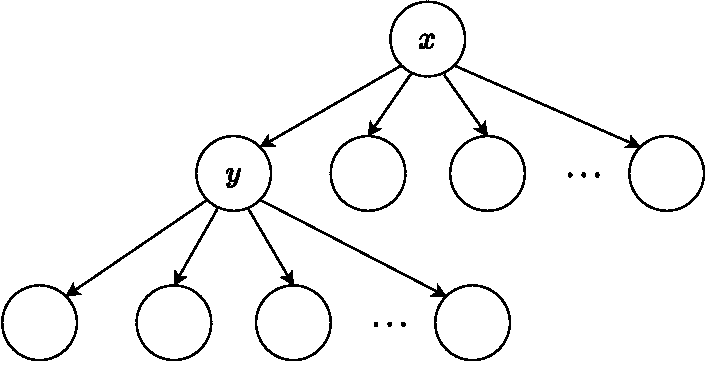
\includegraphics[scale=0.5]{img/link-bitree-xy}
  \caption{如果$x < y$,将$y$作为$x$的第一棵子树。}
  \label{fig:link-xy}
\end{figure}

使用“左侧孩子,右侧兄弟”的实现如下。链接操作可以在常数时间内完成。

\begin{algorithmic}[1]
\Function{Link}{$x, y$}
  \If{\Call{Key}{$y$} $<$ \Call{Key}{$x$}}
    \State Exchange $x \leftrightarrow y$
  \EndIf
  \State \Call{Sibling}{$y$} $\gets$ \Call{Sub-Trees}{$T_1$}
  \State \Call{Sub-Trees}{$x$} $\gets y$
  \State \Call{Parent}{$y$} $\gets x$
  \State \Call{Rank}{$x$} $\gets$ \Call{Rank}{$y$} + 1
  \State \Return $x$
\EndFunction
\end{algorithmic}

\begin{Exercise}
\Question{编程产生帕斯卡三角形}
\Question{证明二项式树$B_n$中第$i$行的节点数为$\binom{n}{i}$。}
\Question{证明二项式树$B_n$中含有$2^n$个节点。}
\Question{用容器保存子树,实现二项式树的链接。这种方式有何问题,怎样解决?}
\end{Exercise}

\begin{Answer}
\Question{编程产生帕斯卡三角形
\begin{Haskell}[frame=single]
pascal = gen [1] where
  gen cs (x:y:xs) = gen ((x + y) : cs) (y:xs)
  gen cs _ = 1 : cs
\end{Haskell}
}
\Question{证明二项式树$B_n$中第$i$行的节点数为$\binom{n}{i}$。
\begin{proof}
使用数学归纳法。$B_0$只有一个根节点。设$B_n$中每行满足二项式系数。树$B_{n+1}$由两棵$B_n$组成。第0行为根节点:$1 = \binom{n+1}{0}$。第$i$行的节点包含两部分,一部分是最左侧子树$B_n$的第$i-1$行,一部分是另一棵$B_n$的第$i$行,总共有:

\[
\begin{array}{rcl}
\binom{n}{i-1} + \binom{n}{i} & = & \dfrac{n!}{(i-1)!(n-i+1)!} + \dfrac{n!}{i!(n-i)!} \\
 & = & \dfrac{n!}{(i-1)!(n-i)!}(\dfrac{1}{i} - \dfrac{1}{n-i+1}) \\
 & = & \dfrac{n!}{(i-1)!(n-i)!}\dfrac{n+1}{i(n-i+1)} \\
 & = & \dfrac{(n+1)!}{i!(n-i+1)!} \\
 & = & \binom{n+1}{i} \\
\end{array}
\]
\end{proof}
}
\Question{证明二项式树$B_n$中含有$2^n$个节点。
\begin{proof}
根据上一练习中证明的结果,$B_n$中各行节点相加为:
\[
\begin{array}{cll}
  & \binom{n}{0} + \binom{n}{1} + ... + \binom{n}{n} & \text{各行相加} \\
= & (1 + 1)^n & \text{令二项式} (a + b)^n \text{中}a = b = 1 \\
= & 2^n & \\
\end{array}
\]
\end{proof}
}
\Question{用容器保存子树,实现二项式树的链接程序。这种方式有何问题,怎样解决?

如果用数组保存子树,在所有元素前插入需要线性时间:

\begin{algorithmic}[1]
\Function{Link'}{$T_1, T_2$}
  \If{\Call{Key}{$T_2$} $<$ \Call{Key}{$T_1$}}
    \State Exchange $T_1 \leftrightarrow T_2$
  \EndIf
  \State \Call{Parent}{$T_2$} $\gets T_1$
  \State \textproc{Insert}(\Call{Sub-Trees}{$T_1$}, 1, $T_2$)
  \State \Call{Rank}{$T_1$} $\gets$ \Call{Rank}{$T_2$} + 1
  \State \Return $T_1$
\EndFunction
\end{algorithmic}

为此,我们可以将子树逆序保存。这样将新树附加到末尾只需要常数时间。
}
\end{Answer}

\subsection{插入}
\index{二项式堆!插入} \index{二项式堆!push}

我们令堆中二项式树按照秩递增排列,并在插入新树时保持秩的顺序:

\be
\begin{array}{rcl}
ins\ t\ [\ ] & = & [t] \\
ins\ t\ (t':ts) & = & \begin{cases}
  rank\ t < rank\ t': & t:t':ts \\
  rank\ t' < rank\ t: & t' : ins\ t\ ts \\
  \text{否则}: & ins\ (link\ t\ t')\ ts  \\
\end{cases}
\end{array}
\ee

其中$rank\ (r, k, ts) = r$,获取一棵二项式树的秩。如果堆为空$[\ ]$,则新树$t$成为堆中唯一的树;否则,我们比较$t$和堆中第一棵树$t'$的秩。如果$t$的秩较小,则$t$成为第一棵树;如果$t'$的秩较小,我们递归地将$t$插入到剩余的树中;如果秩相等,就将$t$、$t'$链接成一棵更大的树,然后递归地插入到剩余的树中。如果有$n$个元素,堆中最多有$O(\lg n)$棵二项式树。$ins$最多执行$O(\lg n)$次常数时间的链接。其时间复杂度为$O(\lg n)$\footnote{这一过程和两个二进制数的加法相似,可以引出一类问题:数值表示(numeric representation)\cite{okasaki-book}。}。使用$ins$,我们可以定义二项式堆的插入算法。先将待插入元素$x$放入一棵只有一个叶子节点树中,然后再插入到堆中:

\be
insert\ x = ins\ (0, x, [\ ])
\ee

这一定义是柯里化的。我们可以利用叠加操作将若干元素插入到堆中:

\be
\textit{fromList} = foldr\ insert\ [\ ]
\ee

对应的“左侧孩子,右侧兄弟”实现如下:\label{alg:insert-tree}

\begin{algorithmic}[1]
\Function{Insert-Tree}{$T, H$}
  \State $\perp \gets p \gets$ \Call{Node}{$0$, NIL, NIL}
  \While{$H \neq$ NIL 且 \Call{Rank}{$H$} $\leq$ \Call{Rank}{$T$}}
    \State $T_1 \gets H$
    \State $H \gets $ \Call{Sibling}{$H$}
    \If{\Call{Rank}{$T$} = \Call{Rank}{$T_1$}}
      \State $T \gets$ \Call{Link}{$T, T_1$}
    \Else
      \State \Call{Sibling}{$p$} $\gets T_1$
      \State $p \gets T_1$
    \EndIf
  \EndWhile
  \State \Call{Sibling}{$p$} $\gets T$
  \State \Call{Sibling}{$T$} $\gets H$
  \State \Return \Call{Remove-First}{$\perp$}
\EndFunction
\Statex
\Function{Remove-First}{$H$}
  \State $n \gets$ \Call{Sibling}{$H$}
  \State \Call{Sibling}{$H$} $\gets$ NIL
  \State \Return $n$
\EndFunction
\end{algorithmic}

\subsection{堆合并}
\index{二项式树!合并}

合并两个二项式堆相当于合并两个二项式树森林。合并结果中没有秩相同的树,并且按照秩递增。合并过程和归并排序类似。每次从两个堆中各取出第一棵树,比较它们的秩,将较小的一棵放入结果中。如果两棵树的秩相等,我们将它们链接成为一棵较大的树,然后递归插入到合并结果中。

\be
\begin{array}{rcl}
merge\ ts_1\ [\ ] & = & ts_1 \\
merge\ [\ ]\ ts_2 & = & ts_2 \\
merge\ (t_1:ts_1)\ (t_2:ts_2) & = & \begin{cases}
  rank\ t_1 < rank\ t_2: & t_1 : (merge\ ts_1\ (t_2:ts_2)) \\
  rank\ t_2 < rank\ t_1: & t_2 : (merge\ (t_1:ts_1)\ ts_2) \\
  \text{否则}: & ins\ (link\ t_1\ t_2)\ (merge\ ts_1\ ts_2) \\
  \end{cases}
\end{array}
\ee

当$t_1$、$t_2$秩相同时,我们也可以将链接后的树插入回任意一个堆,然后递归合并:

\[
merge\ (ins\ (link\ t_1\ t_2)\ ts_1)\ ts_2
\]

用这种方式可以消除递归,用迭代的方式实现堆合并:

\begin{algorithmic}[1]
\Function{Merge}{$H_1, H_2$}
  \State $H \gets p \gets$ \Call{Node}{0, NIL, NIL}
  \While{$H_1 \neq$ NIL 且 $H_2 \neq$ NIL}
    \If{\Call{Rank}{$H_1$} $<$ \Call{Rank}{$H_2$}}
      \State \Call{Sibling}{$p$} $\gets H_1$
      \State $p \gets$ \Call{Sibling}{$p$}
      \State $H_1 \gets$ \Call{Sibling}{$H_1$}
    \ElsIf{\Call{Rank}{$H_2$} $<$ \Call{Rank}{$H_1$}}
      \State \Call{Sibling}{$p$} $\gets H_2$
      \State $p \gets$ \Call{Sibling}{$p$}
      \State $H_2 \gets$ \Call{Sibling}{$H_2$}
    \Else \Comment{秩相等}
      \State $T_1 \gets H_1, T_2 \gets H_2$
      \State $H_1 \gets$ \Call{Sibling}{$H_1$}, $H_2 \gets$ \Call{Sibling}{$H_2$}
      \State $H_1 \gets $ \textproc{Insert-Tree}(\Call{Link}{$T_1, T_2$}, $H_1$)
    \EndIf
  \EndWhile
  \If{$H_1 \neq$ NIL}
    \State \Call{Sibling}{$p$} $\gets H_1$
  \EndIf
  \If{$H_2 \neq$ NIL}
    \State \Call{Sibling}{$p$} $\gets H_2$
  \EndIf
  \State \Return \Call{Remove-First}{$H$}
\EndFunction
\end{algorithmic}

设堆$H_1$中有$m_1$棵树,堆$H_2$中有$m_2$棵树。合并后的结果中最多有$m_1 + m_2$棵树。如果没有秩相同的树,则合并时间为$O(m_1 + m_2)$。如果存在秩相同的树,最多需要调用$O(m_1 + m_2)$次$ins$。考虑$m_1 = 1 + \lfloor \lg n_1 \rfloor$,$m_2 = 1 + \lfloor \lg n_2 \rfloor$,其中$n_1$和$n_2$是两个堆各自的元素数,且$\lfloor \lg n_1 \rfloor + \lfloor \lg n_2 \rfloor \leq 2 \lfloor \lg n \rfloor$,其中$n = n_1 + n_2$。最终合并的复杂度为$O(\lg n)$。

\subsection{弹出}
\index{二项式堆!弹出}

二项式堆中,每棵树的根节点保存了树中的最小元素。但根节点元素间的大小关系是任意的。为了获取堆中的最小元素,需要在全部根节点中查找。因为堆中有$O(\lg n)$棵树,所以获取最小值的时间复杂度为$O(\lg n)$。但是弹出操作不仅找出最小元素,还需要将其删除并保持堆性质。设堆中的二项式树为$B_i, B_j, ..., B_p, ..., B_m$。设$B_p$的根节点为堆中最小元素。将其删除后会产生$p$棵子二项式树,秩为$p-1, p-2, ..., 0$。我们可以将$p$棵子树逆序,形成一个新二项式堆$H_p$。除去$B_p$的树也构成一个二项式堆$H' = H - [B_p]$。将$H_p$和$H'$合并就可以得到最终结果,如图\cref{fig:bheap-del-min}所示。我们首先定义从堆中寻找最小元素的操作:

\begin{figure}[htbp]
  \centering
  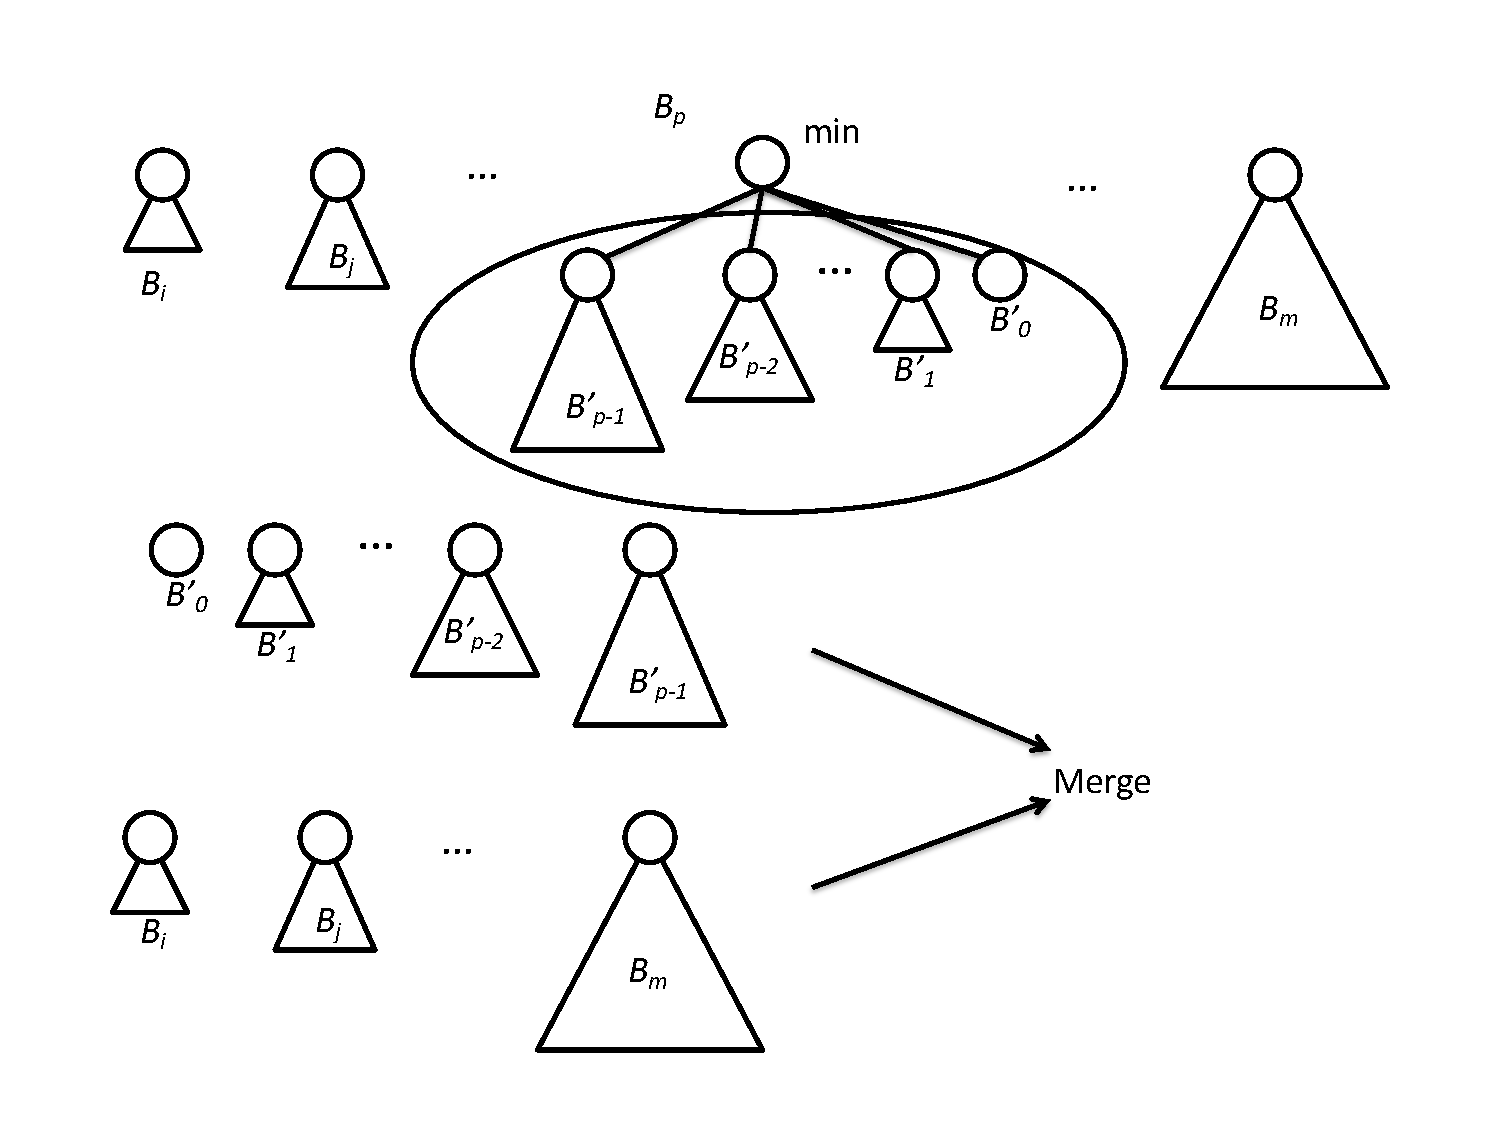
\includegraphics[scale=0.4]{img/bheap-pop}
  \caption{二项式堆的弹出操作}
  \label{fig:bheap-del-min}
\end{figure}

\be
top\ (t:ts) = foldr\ f\ (key\ t)\ ts
\ee

其中

\[
f\ (r, x, ts)\ y = min\ x\ y
\]

这相当于遍历堆中的所有树,找出根节中存储的最小值:

\begin{algorithmic}[1]
\Function{Top}{$H$}
  \State $m \gets \infty$
  \While{$H \neq$ NIL}
    \State $m \gets$ \textproc{Min}($m$, \Call{Key}{$H$})
    \State $H \gets $ \Call{Sibling}{$H$}
  \EndWhile
  \State \Return $m$
\EndFunction
\end{algorithmic}

为了实现弹出,我们需要从堆中分离出最小元素所在的树:

\be
\begin{array}{rcl}
min'\ [t] & = & (t, [\ ]) \\
min'\ (t:ts) & = & \begin{cases}
  key\ t < key\ t': & (t, ts), \text{其中}: (t', ts') = min'\ ts \\
  \text{否则}: & (t', t:ts')
  \end{cases}
\end{array}
\label{eq:extract-min-bitree}
\ee

其中$key\ (r, k, ts) = k$获取二项式树中的根节点元素。$min'$的结果为一对值:最小元素所在的树,和其它的树。接下来就可以定义弹出操作:

\be
pop\ H = (k, merge\ (reverse\ ts)\ H'), \text{其中}: ((r, k, ts), H') = min'\ H
\ee

对应的迭代实现为:

\begin{algorithmic}[1]
\Function{Pop}{$H$}
  \State $(T_m, H) \gets$ \Call{Extract-Min}{$H$}
  \State $H \gets$ \textproc{Merge}($H$, \textproc{Reverse}(\Call{Sub-Trees}{$T_m$}))
  \State \Call{Sub-Trees}{$T_m$}
  \State \Return (\Call{Key}{$T_m$}, $H$)
\EndFunction
\end{algorithmic}

其中反转操作的实现见第一章,\textproc{Extract-Min}的迭代实现如下:

\begin{algorithmic}[1]
\Function{Extract-Min}{$H$}
  \State $H' \gets H, p \gets$ NIL
  \State $T_m \gets T_p \gets$ NIL
  \While{$H \neq$ NIL}
    \If{$T_m =$ NIL 或 \Call{Key}{$H$} $<$ \Call{Key}{$T_m$}}
      \State $T_m \gets H$
      \State $T_p \gets p$
    \EndIf
    \State $p \gets H$
    \State $H \gets $ \Call{Sibling}{$H$}
  \EndWhile
  \If{$T_p \neq$ NIL}
    \State \Call{Sibling}{$T_p$} $\gets$ \Call{Sibling}{$T_m$}
  \Else
    \State $H' \gets$ \Call{Sibling}{$T_m$}
  \EndIf
  \State \Call{Sibling}{$T_m$} $\gets$ NIL
  \State \Return $(T_m, H')$
\EndFunction
\end{algorithmic}

使用弹出操作可以实现堆排序。首先从待排序元素构建一个二项式堆,然后不断从中弹出最小元素。

\be
sort  = heapSort \circ fromList
\ee

其中$heapSort$实现如下:

\be
\begin{array}{rcl}
  heapSort\ [\ ] & = & [\ ] \\
  heapSort\ H & = & k : (heapSort\ H'), \text{其中}: (k, H') = pop\ H
\end{array}
\ee

二项式堆的插入、合并的时间复杂度在最坏情况下是$O(\lg n)$。他们的分摊复杂度为常数时间,我们这里略去了分摊复杂度的证明。

\section{斐波那契堆}
\label{fib-heap} \index{斐波那契堆}

二项式堆的名字来自二项式展开,斐波那契堆的名字来自斐波那契数列\footnote{Michael L. Fredman和Robert E. Tarjan在证明这种堆的时间复杂度时使用了斐波那契数列的性质,他们于是给这种堆命名为“斐波那契堆”\cite{CLRS}。}。斐波那契堆本质上是一个惰性二项式堆。但这并不意味着二项式堆在支持惰性求值的环境下自动就成为了斐波那契堆。惰性环境仅提供了实现上的便利\cite{hackage-fibq}。除弹出操作外,斐波那契堆所有操作的分摊复杂度都可以达到常数时间\cite{okasaki-fibh}。

\begin{table}[htbp]
\centering
\begin{tabular}{| l | c | r |}
  \hline
  操作 & 二项式堆 & 斐波那契堆 \\
  \hline
  插入 & $O(\lg n)$ & $O(1)$ \\
  \hline
  合并 & $O(\lg n)$ & $O(1)$ \\
  \hline
  获取堆顶 & $O(\lg n)$ & $O(1)$ \\
  \hline
  弹出 & $O(\lg n)$ & 分摊 $O(\lg n)$ \\
  \hline
\end{tabular}
\caption{斐波那契堆和二项式堆的(分摊)复杂度对比}
\end{table}

向二项式堆插入新元素$x$时,我们将$x$放入只有一个叶子节点的树中,然后插入到森林中。树按照秩递增的顺序插入,如果秩相等,则进行链接,然后递归插入。时间复杂度为$O(\lg n)$。使用惰性策略,我们将按秩有序插入和链接等操作推迟进行。将$x$所在的树直接加入森林中。为了快速获得堆顶元素,我们需要记录哪一棵树的根节点保存了最小元素。一个斐波那契堆或者为空$\nil$,或者是若干树的森林,记为$(n, t_m, ts)$。其中含有最小元素的树被单独记录为$t_m$,堆中元素个数记录为$n$,其余二项式树的列表为$ts$。下面的例子程序定义了斐波那契堆(复用了二项式树的定义):

\begin{lstlisting}[style=Haskell]
data FibHeap a = E | FH { size :: Int
                        , minTree :: BiTree a
                        , trees :: [BiTree a]}
\end{lstlisting}

这样就可以用常数时间获取堆顶元素:$top\ H = key\ \textit{minTree}\ H$。

\subsection{插入}
\index{斐波那契堆!插入}

我们将插入定义为一种特殊的合并操作,其中一个堆仅含有一棵一个叶节点的树:

\[
insert\ x\ H = merge\ (singleton\ x)\ H
\]

或写成柯里化的形式:

\be
insert = merge \circ singleton
\label{eq:fib-insert}
\ee

其中$singleton$从$x$构建仅含有一个元素的树:

\[
singleton\ x = (1, (1, x, [\ ]), [\ ])
\]

插入操作也可以实现为向森林中追加一个新节点,然后更新存有最小元素的树。

\begin{algorithmic}[1]
\Function{Insert}{$k, H$}
  \State $x \gets$ \Call{Singleton}{$k$} \Comment{将$k$装入一棵树}
  \State \textproc{Add}($x$, \Call{Trees}{$H$})
  \State $T_m \gets$ \Call{Min-Tree}{$H$}
  \If{$T_m = $ NIL 或 $k <$ \Call{Key}{$T_m$}}
    \State \Call{Min-Tree}{$H$} $\gets x$
  \EndIf
  \State \Call{Size}{$H$} $\gets$ \Call{Size}{$H$} + 1
\EndFunction
\end{algorithmic}

其中\textproc{Trees}($H$)获取堆$H$中所有树的列表,\textproc{Min-Tree}($H$)记录了$H$中最小元素所在的树。

\subsection{合并}
\index{斐波那契堆!合并}

和二项式堆不同,我们在合并时将链接操作推迟到将来,仅仅将两个堆中的树放到一起,然后比较出新的含有最小元素的树。

\be
\begin{array}{rcl}
merge\ h\ \nil & = & h \\
merge\ \nil\ h & = & h \\
merge\ (n, t_m, ts)\ (n', t_m', ts') & = & \begin{cases}
  key\ t_m < key\ t_m': & (n + n', t_m, t_m' : ts \doubleplus ts') \\
  \text{否则}: & (n + n', t_m', t_m : ts \doubleplus ts') \\
  \end{cases}
\end{array}
\ee

当两个堆都不为空时,这一实现中的$\doubleplus$操作和其中一个堆中树的棵数成正比。如果使用双向链表,则可以把堆合并操作提高到常数时间。下面的例子程序使用双向链表定义了斐波那契堆:

\begin{lstlisting}[language = Bourbaki]
data Node<K> {
    K key
    Int rank
    Node<k> next, prev, parent, subTrees
}

data FibHeap<K> {
    Int size
    Node<K> minTree, trees
}
\end{lstlisting}

这样就可以实现常数时间的合并操作:

\begin{algorithmic}[1]
\Function{Merge}{$H_1, H_2$}
  \State $H \gets$ \Call{Fib-Heap}{}
  \State \Call{Trees}{$H$} $\gets$ \textproc{Concat}(\Call{Trees}{$H_1$}, \Call{Trees}{$H_2$})
  \If{\textproc{Key}(\Call{Min-Tree}{$H_1$}) $<$ \textproc{Key}(\Call{Min-Tree}{$H_2$})}
    \State \Call{Min-Tree}{$H$} $\gets$ \Call{Min-Tree}{$H_1$}
  \Else
    \State \Call{Min-Tree}{$H$} $\gets$ \Call{Min-Tree}{$H_2$}
  \EndIf
  \Call{Size}{$H$} = \Call{Size}{$H_1$} + \Call{Size}{$H_2$}
  \State \Return $H$
\EndFunction
\Statex
\Function{Concat}{$s_1, s_2$}
  \State $e_1 \gets$ \Call{Prev}{$s_1$}
  \State $e_2 \gets$ \Call{Prev}{$s_2$}
  \State \Call{Next}{$e_1$} $\gets s_2$
  \State \Call{Prev}{$s_2$} $\gets e_1$
  \State \Call{Next}{$e_2$} $\gets s_1$
  \State \Call{Prev}{$s_1$} $\gets e_2$
  \State \Return $s_1$
\EndFunction
\end{algorithmic}

\subsection{弹出}
\index{斐波那契堆!弹出} \index{斐波那契堆!删除最小元素}

我们在合并时推迟了树的链接,接下来需要在弹出时将其“补偿”回来。我们定义这一过程为树的归并。首先考虑这样一个问题:给定若干2的整数次幂,如:$L = [2, 1, 1, 4, 8, 1, 1, 2, 4]$,我们不断将值相同的两个数字相加,直到没有任何相等的数。这个例子的最终结果为$[8, 16]$。表\cref{tb:num-consolidate}给出了归并的步骤。第一列表示每次“扫描”到的数字;第二列是中间结果。被扫描的数字和结果列表中的第一个元素相比较。如果相等,就用两个括号围起来;最后一列是归并的结果,每个结果都用于下一步的处理。这个数的归并的过程可以用叠加来实现:

\begin{table}[htbp]
\centering
\begin{tabular}{| r | l | l |}
  \hline
  数字 & 比较、相加 & 结果 \\
  \hline
  2 & 2 & 2 \\
  \hline
  1 & 1, 2 & 1, 2 \\
  \hline
  1 & (1+1), 2 & 4 \\
  \hline
  4 & (4+4) & 8 \\
  \hline
  8 & (8+8) & 16 \\
  \hline
  1 & 1, 16 & 1, 16 \\
  \hline
  1 & (1+1), 16 & 2, 16 \\
  \hline
  2 & (2+2), 16 & 4, 16 \\
  \hline
  4 & (4+4), 16 & 8, 16 \\
  \hline
\end{tabular}
\caption{归并数字的步骤}
\label{tb:num-consolidate}
\end{table}

\be
consolidate = foldr\ melt\ [\ ]
\ee

其中$melt$定义为:

\be
\begin{array}{rcl}
  melt\ x\ [\ ] & = & x \\
  melt\ x\ (x':xs) & = & \begin{cases}
    x = x': & melt\ 2x\ xs \\
    x < x': & x : x' : xs \\
    x > x': & x' : melt\ x\ xs \\
  \end{cases}
\end{array}
\ee

令$n = sum\ L$,为所有数字的和,$consolidate$相当于把$n$表示为二进制数,如果第$i$位上的数字是1,则最终列表中包含$2^i$这个数($i$从0开始)。例如$sum [2, 1, 1, 4, 8, 1, 1, 2, 4] = 24$,写成二进制是11000,第3和第4位上是1,所以最终列表中包含$2^3= 8, 2^4 = 16$。用类似的方法可以实现树的归并。我们需要比较秩,并把秩相同的树链接起来:

\be
\begin{array}{rcl}
  melt\ t\ [\ ] & = & [t] \\
  melt\ t\ (t':ts) & = & \begin{cases}
    rank\ t = rank\ t': & melt\ (link\ t\ t')\ ts \\
    rank\ t < rank\ t': & t : t' : ts \\
    rank\ t > rank\ t': & t' : melt\ t\ ts \\
  \end{cases}
\end{array}
\ee

图\cref{fig:fib-melt-b}给出了斐波那契堆树归并过程的步骤,和表\cref{tb:num-consolidate}对比可以看出它们是相似的。我们也可以使用一个辅助数组$A$来进行归并。$A[i]$保存秩为$i$的树。在遍历堆中的树时,如果遇到另一棵秩为$i$的树,我们就将它们链接起来得到一棵秩为$i+1$的树。然后将$A[i]$清空,并接着检查$A[i+1]$是否为空,若不为空,就再次进行链接。遍历完成后,$A$中就保存了归并后的结果。

\captionsetup[subfigure]{labelformat=empty, margin=10pt}
\begin{figure}[htbp]
  \centering
  \subcaptionbox{归并前}{\includegraphics[scale=0.35]{img/fib-meld-01}} \\
  \subcaptionbox{第1、2步}{\includegraphics[scale=0.35]{img/fib-meld-02}\hspace{0.1\textwidth}}
  \subcaptionbox{第3步,d先链接到c,然后链接到a。}{ \hspace{0.1\textwidth} \includegraphics[scale=0.35]{img/fib-meld-03} \hspace{0.1\textwidth}}
  \subcaptionbox{第4步}{\includegraphics[scale=0.35]{img/fib-meld-04}}\\
  \subcaptionbox{第5步}{\includegraphics[scale=0.35]{img/fib-meld-05}}
  \subcaptionbox{第6步}{\includegraphics[scale=0.35]{img/fib-meld-06}} \\
  \subcaptionbox{第7、8步,r先链接到q,然后s链接到q。}{\includegraphics[scale=0.35]{img/fib-meld-07}}
  \caption{树归并的步骤}
  \label{fig:fib-melt-b}
\end{figure}
\captionsetup[subfigure]{labelformat=parens}

\begin{algorithmic}[1]
\Function{Consolidate}{$H$}
  \State $R \gets $ \textproc{Max-Rank}(\Call{Size}{$H$})
  \State $A \gets$ [NIL, NIL, ..., NIL] \Comment{共$R$个}
  \For{each $T$ in \Call{Trees}{$H$}}
    \State $r \gets $ \Call{Rank}{$T$}
    \While{$A[r] \neq$ NIL}
      \State $T' \gets A[r]$
      \State $T \gets $ \Call{Link}{$T, T'$}
      \State $A[r] \gets$ NIL
      \State $r \gets r + 1$
    \EndWhile
    \State $A[r] \gets T$
  \EndFor
  \State $T_m \gets$ NIL
  \State \Call{Trees}{$H$} $\gets$ NIL
  \For{each $T$ in $A$}
    \If{$T \neq$ NIL}
      \State append $T$ to \Call{Trees}{$H$}
      \If{$T_m = NIL$ or \Call{Key}{$T$} $<$ \Call{Key}{$T_m$}}
        \State $T_m \gets T$
      \EndIf
    \EndIf
  \EndFor
  \State \Call{Min-Tree}{$H$} $\gets T_m$
\EndFunction
\end{algorithmic}

%% 用上述算法处理图\cref{fig:fib-meld-a}中所示的斐波那契堆,各个步骤中的数组$A$如图\cref{fig:fib-cons-c}所示。

%% \captionsetup[subfigure]{labelformat=empty, margin=10pt}
%% \begin{figure}[htbp]
%%   \centering
%%   \subcaptionbox{第1、2步}{\includegraphics[scale=0.35]{img/fib-cons-02}}
%%   \subcaptionbox{第3步,因为$A_0 \neq NIL$,‘d’先被链接到‘c’,然后$A_0$被清除为NIL。接下来,由于$A_1 \neq NIL$,‘c’被链接到‘a’,新的树被存入$A_2$。}{\hspace{0.1\textwidth}\includegraphics[scale=0.35]{img/fib-cons-03}\hspace{0.1\textwidth}}
%%   \subcaptionbox{第4步}{\includegraphics[scale=0.35]{img/fib-cons-04}} \\
%%   \subcaptionbox{第5步}{\includegraphics[scale=0.35]{img/fib-cons-05}}
%%   \subcaptionbox{第6步}{\includegraphics[scale=0.35]{img/fib-cons-06}} \\
%%   \subcaptionbox{第7、8步,因为$A_0 \neq NIL$,‘r’被链接到‘q’,新树存入$A_1$($A_0$清空);接着‘s’链接到‘q’,并存入$A_2$($A_1$清空)。}{\includegraphics[scale=0.35]{img/fib-cons-07}}
%%   \caption{树归并的步骤} \label{fig:fib-cons-c}
%% \end{figure}
%% \captionsetup[subfigure]{labelformat=parens}

将堆中所有二项式树归并后,斐波那契堆就变成了二项式堆。此时堆中的树合并为$O(\lg n)$棵。\textproc{Max-Rank}($n$)返回$n$个元素的堆中最大可能的秩$R$。根据二项式堆的结论,秩最大的树$B_R$有$2^R$个元素。我们有:$2^R \leq n < 2^{R+1}$。
我们推测它一个大致上限为$R \leq \log_2 n$。我们稍后给出$R$的更准确的估计。我们需要额外扫描一遍所有树的根节点,找到存有最小元素的树。我们可以复用(\cref{eq:extract-min-bitree})定义的$min'$分离出堆顶元素所在的树。

\be
\begin{array}{rcl}
  pop\ (1, (0, x, [\ ]), [\ ]) & = & (x, [\ ]) \\
  pop\ (n, (r, x, ts_m), ts) & = & (x, (n - 1, t_m, ts')) \\
\end{array}
\ee

其中$(t_m, ts') = min'\ consolidate\ (ts_m \doubleplus ts)$。注意到$\doubleplus$的时间复杂度是$O(|ts_m|)$,和最小值所在的树中的子树棵数成正比。对应的命令式实现如下:

\begin{algorithmic}[1]
\Function{Pop}{$H$}
  \State $T_m \gets $ \Call{Min-Tree}{$H$}
  \For{each $T$ in \Call{Sub-Trees}{$T_m$}}
    \State append $T$ to \Call{Trees}{$H$}
    \State \Call{Parent}{$T$} $\gets$ NIL
  \EndFor
  \State remove $T_m$ from \Call{Trees}{$H$}
  \State \Call{Size}{$H$} $\gets$ \Call{Size}{$H$} - 1
  \State \Call{Consolidate}{$H$}
  \State \Return (\Call{Key}{$T_m$}, $H$)
\EndFunction
\end{algorithmic}

我们使用“势能方法”分析弹出算法的分摊性能。回忆物理学中重力势能的定义:

\be
E = m g h
\ee

如图\cref{fig:potential-energy}所示,假设一个复杂的操作过程,将质量为$m$的物体上下移动,最终物体静止在了高为$h'$的位置。如果这一过程中的摩擦阻力做功$W_f$,则做功的总和为:

\[
W = m g (h' - h) + W_f
\]

\begin{figure}[htbp]
  \centering
  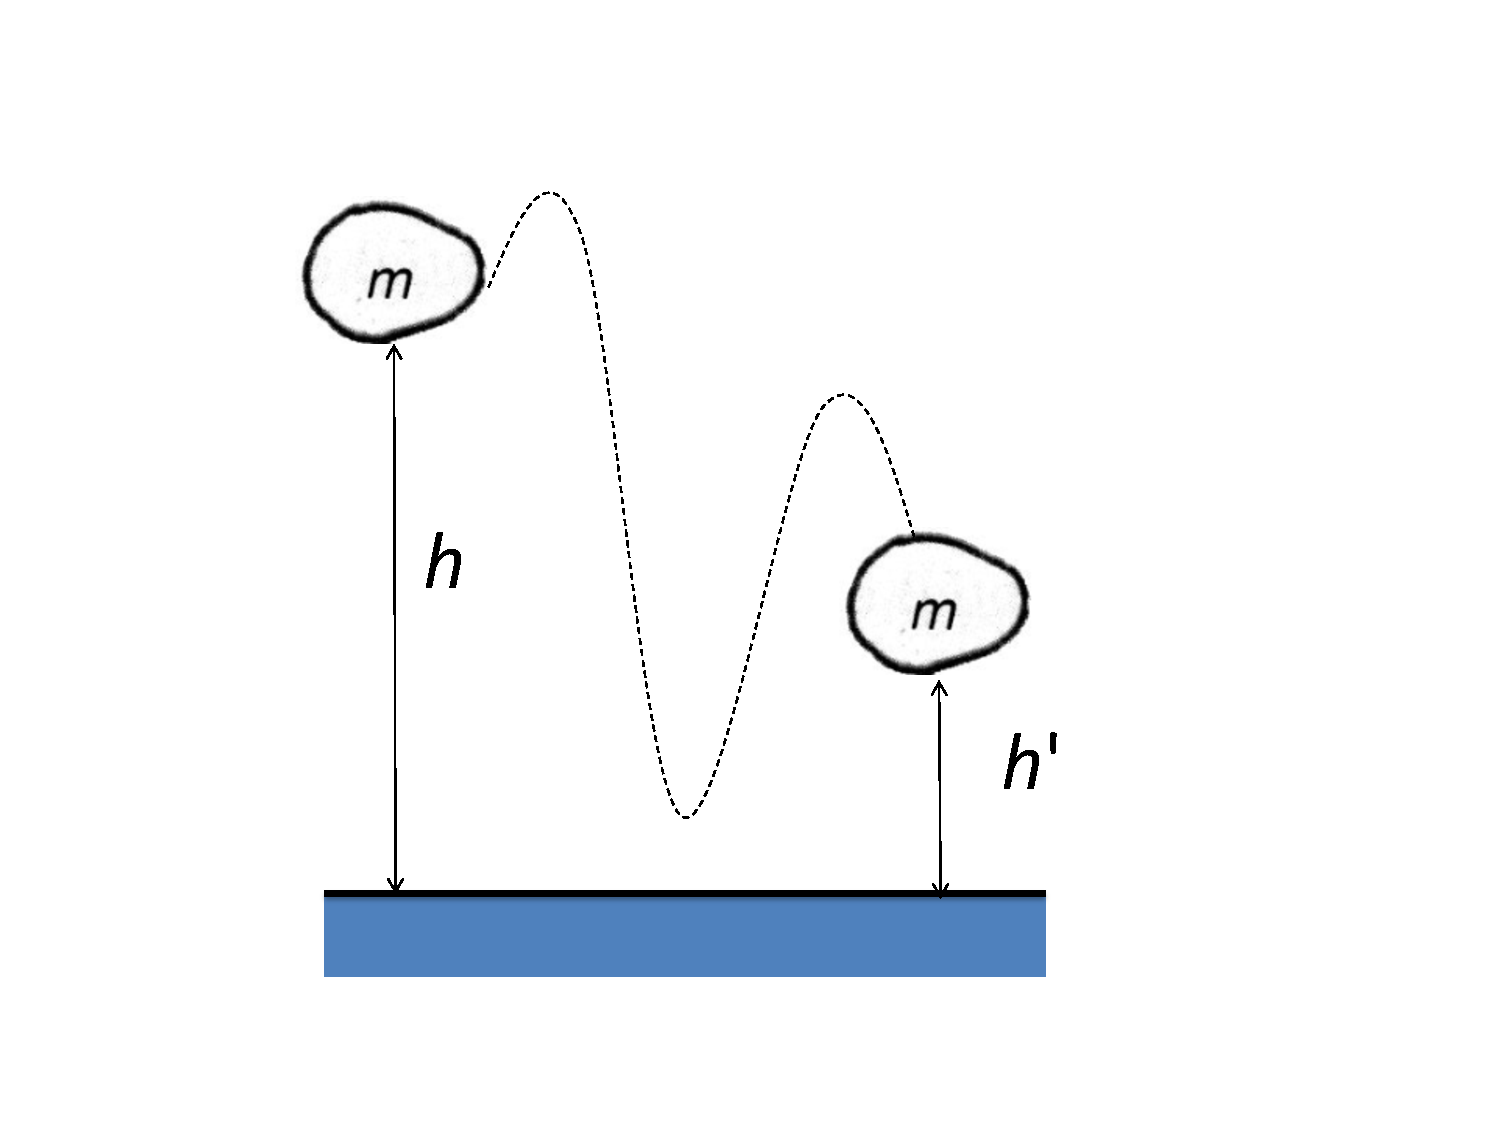
\includegraphics[scale=0.35]{img/potential-energy}
  \caption{重力势能}
  \label{fig:potential-energy}
\end{figure}

考虑斐波那契堆的弹出操作。为了计算总消耗,我们首先定义删除最小元素前的势能为$\Phi(H)$。这个势能是由迄今为止的插入、合并操作累积的。经过树的归并,形成了新的堆$H'$,由此计算新的势能$\Phi(H')$。$\Phi(H')$和$\Phi(H)$的差再加上树归并消耗的部分就可以给出弹出的分摊复杂度。定义势能为:

\be
\Phi(H) = t(H)
\ee

其中$t(H)$是堆中树的棵数。对于$n$个节点的斐波那契堆,令堆中所有树秩的上限为$R(n)$。归并后,堆中树的棵数最多为$t(H') = R(n) + 1$。在归并前,我们还做了另外一个重要的操作,也对总运行时间有所贡献:我们将存有最小元素的树根删除,然后将其全部子树添加到森林中。因此树归并操作最多处理$R(n) + t(H) - 1$棵树。设弹出操作的时间复杂度为$T$,树归并的时间复杂度为$T_c$,我们推导分摊性能如下:

\be
\begin{array}{rcl}
T & = & T_c + \Phi(H') -\Phi(H) \\
  & = & O(R(n) + t(H) - 1) + (R(n) + 1) - t(H) \\
  & = & O(R(n))
\end{array}
\ee

插入、合并、弹出操作可以确保斐波那契堆中的所有树都为二项式树,此时$R(n)$的上限为$O(\lg n)$。

\subsection{提升优先级}
\index{斐波那契堆!提升优先级}

提升优先级是堆的一个实际应用。用堆管理若干任务,某个任务需要提前执行,为此我们希望将代表其优先级的数值减小,使得任务更接近堆顶。某些图算法,例如最小生成树算法和Dijkstra算法都依赖这一操作\cite{CLRS}。并且我们需要其分摊性能达到常数时间。令$x$指向堆$H$中的某个节点,我们希望将它的值减小为$k$。如图\cref{fig:cut-fib-tree},若节点$x$的值小于父节点$y$,将子树$x$切下并添加到堆(森林)中。尽管这样可以使得每棵树的父节点仍然存有最小值,但切除节点后的树不再是二项式树。如果失去了很多子树,就无法保证合并操作的性能。为了解决这一问题,我们给斐波那契堆增加一个限制条件:

\begin{center}当一个节点第二次失去了某个子节点时,立即将它切下并添加到堆(森林)中。
\end{center}

\begin{figure}[htbp]
  \centering
  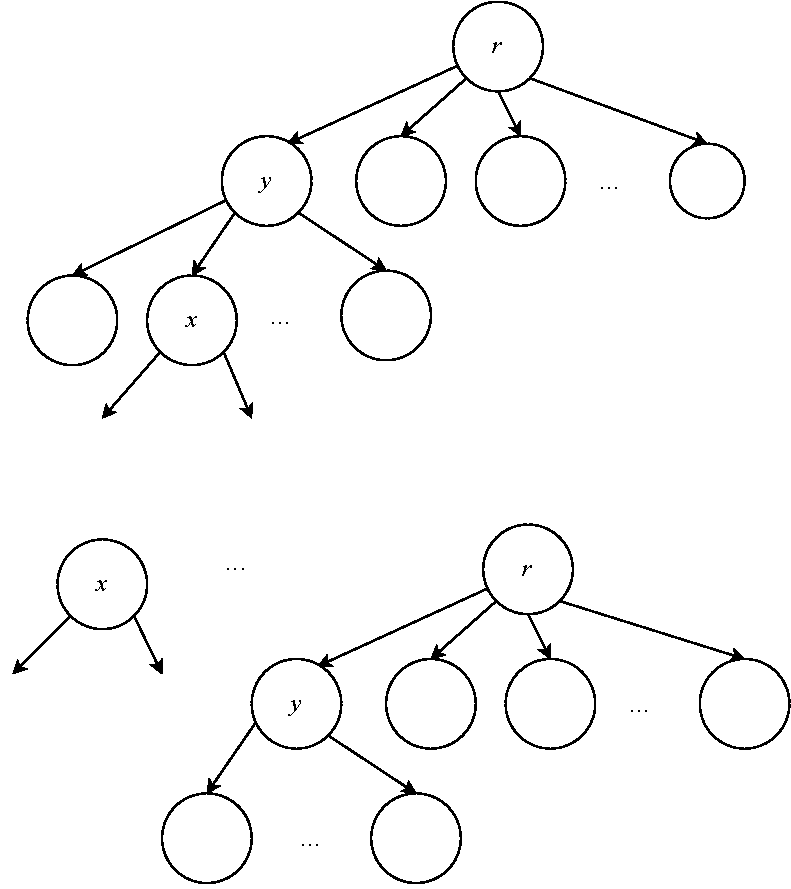
\includegraphics[scale=0.5]{img/fib-cut-past}
  \caption{若$key\ x < key\ y$,将$x$切下,然后添加到堆中。}
  \label{fig:cut-fib-tree}
\end{figure}

\begin{algorithmic}[1]
\Function{Decrease}{$H, x, k$}
  \State \Call{Key}{$x$} $\gets k$
  \State $p \gets $ \Call{Parent}{$x$}
  \If{$p \neq$ NIL and $k < $ \Call{Key}{$p$}}
    \State \Call{Cut}{$H, x$}
    \State \Call{Cascade-Cut}{$H, p$} \Comment{回溯切除}
  \EndIf
  \If{$k <$ \Call{Top}{$H$}}
    \State \Call{Min-Tree}{$H$} $\gets x$
  \EndIf
\EndFunction
\end{algorithmic}

\textproc{Cascade-Cut}使用一个标记来记录它此前是否失去过子节点。并在\textproc{Cut}中清除这一标记。

\begin{algorithmic}[1]
\Function{Cut}{$H, x$}
  \State $p \gets $ \Call{Parent}{$x$}
  \State remove $x$ from $p$
  \State \Call{Rank}{$p$} $\gets$ \Call{Rank}{$p$} - 1
  \State add $x$ to \Call{Trees}{$H$}
  \State \Call{Parent}{$x$} $\gets$ NIL
  \State \Call{Mark}{$x$} $\gets$ False
\EndFunction
\end{algorithmic}

回溯切除时,若节点$x$被标记了,说明它此前已经失去了子节点。我们需要继续回溯切除,直到根节点。

\begin{algorithmic}[1]
\Function{Cascade-Cut}{$H, x$}
  \State $p \gets $ \Call{Parent}{$x$}
  \If{$p \neq$ NIL}
    \If{\Call{Mark}{$x$} $= $ False}
      \State \Call{Mark}{$x$} $\gets$ True
    \Else
      \State \Call{Cut}{$H, x$}
      \State \Call{Cascade-Cut}{$H, p$}
    \EndIf
  \EndIf
\EndFunction
\end{algorithmic}

\begin{Exercise}
证明\textproc{Decrease}的分摊复杂度为常数时间$O(1)$。
\end{Exercise}

\subsection{斐波那契堆的命名}

我们尚未给出\textproc{Max-Rank}($n$)的实现。它定义了$n$个元素的斐波那契堆中所有树的秩的上限。

\begin{lemma}
\label{lemma:Fib-degree}
对于斐波那契堆中的任何树$x$,若其秩为$k$,(即:$k = rank(x)$),$|x|$为树中元素个数,则:

\be
  |x| \geq F_{k+2}
\ee

其中$F_k$为斐波那契数列中的第$k$项:

\[
\begin{array}{rcl}
F_0 & = & 0 \\
F_1 & = & 1 \\
F_k & = & F_{k-1} + F_{k-2} \\
\end{array}
\]
\end{lemma}

\begin{proof}[证明]
考虑节点$x$的全部$k$棵子树:$y_1, y_2, ..., y_k$。顺序是被链接到$x$的时间先后。其中$y_1$最早加入,$y_k$最新加入。显然有$|y_i| \geq 0$。当$y_i$链接到$x$的时候,子树$y_1, y_2, ..., y_{i-1}$已经存在了。因为我们只把秩相同的树链接起来,所以在这一时刻,有:

\[
  rank(y_i) = rank(x) = i - 1
\]

此后$y_i$最多只能失去一个子节点(通过\textproc{Decrease}),一旦失去第二个子节点,它会被立即切除并加入到森林中。因此我们可以推断,对任何$i = 2, 3, ..., k$,有:

\[
rank(y_i) \geq i - 2
\]

令$s_k$为$x$的子节点个数\textbf{可能的最小值},其中$k = rank(x)$。对于边界情况,有$s_0 = 1$, $s_1 = 2$。也就是说:秩为0的树,最少有1个节点,秩为1的树最少有2个节点,秩为$k$的树,最少有$s_k$个节点:

\bea*{rcl}
|x| & \geq & s_k \\
    & =   & 2 + s_{rank(y_2)} + s_{rank(y_3)} + ... + s_{rank(y_k)} \\
    & \geq & 2 + s_0 + s_1 + ... + s_{k-2} \\
\eea*

其中最后一行成立是因为$rank(y_i) \geq i - 2$并且$s_k$单调增,所以$s_{rank(y_i)} \geq s_{i-2}$。我们接下来要证明$s_k > F_{k+2}$。使用数学归纳法。对于边界情况,我们有$s_0 = 1 \geq F_2 = 1$,以及$s_1 = 2 \geq F_3 = 2$。对于$k \geq 2$的情况,我们有:

\bea*{rcll}
|x| & \geq & s_k & \\
    & \geq & 2 + s_0 + s_1 + ... + s_{k-2} & \\
    & \geq & 2 + F_2 + F_3 + ... + F_k & \text{归纳假设}\\
    & =    & 1 + F_0 + F_1 + F_2 + ... + F_k & \text{利用}F_0 = 0, F_1 = 1 \\
\eea*

现在,我们需要证明

\be
F_{k+2} = 1 +  \sum_{i=0}^{k} F_i
\ee

再次使用数学归纳法:

\begin{itemize}
\item 边界情况:$F_2 = 1 + F_0 = 2$
\item 递归情况,假设$k+1$时成立。
\bea*{rcll}
  F_{k+2} & = & F_{k+1} + F_k & \\
         & = & (1 + \displaystyle \sum_{i=0}^{k-1}F_i) + F_k & \text{归纳假设} \\
         & = & 1 + \displaystyle \sum_{i=0}^{k} F_i & \\
\eea*
\end{itemize}

综上,我们得到最终结论:
\be
n \geq |x| \geq F_{k+2}
\ee
\end{proof}

根据斐波那契数列的性质:$F_k \geq \phi^k$,其中$\phi = \dfrac{1+\sqrt{5}}{2}$为黄金分割比。我们同时证明了弹出操作的分摊复杂度为$O(\lg n)$。根据这一结果,我们可以定义$maxRank$为:

\be
  maxRank(n) = 1 + \lfloor \log_{\phi} n \rfloor
\ee

或者利用斐波那契数列的递归定义实现\textproc{Max-Rank}:

\begin{algorithmic}[1]
\Function{Max-Rank}{$n$}
  \State $F_0 \gets 0, F_1 \gets 1$
  \State $k \gets 2$
  \Repeat
    \State $F_k \gets F_{k_1} + F_{k_2}$
    \State $k \gets k + 1$
  \Until{$F_k < n$}
  \State \Return $k - 2$
\EndFunction
\end{algorithmic}

\section{配对堆}
\label{pairing-heap} \index{配对堆}

斐波那契堆的实现较为复杂。本节介绍配对堆。它实现简单、性能优异。大部分操作,包括插入、获取堆顶、合并都是常数时间复杂度,人们猜测它的弹出操作的分摊复杂度为$O(\lg n)$\cite{pairing-heap}\cite{okasaki-book}。

\subsection{定义}
\index{配对堆!定义}

配对堆实现为一棵多叉树。最小元素保存于树根。一个配对堆要么为空$\nil$,要么是一棵$k$叉树,包含一个根节点和一组子树,记为$(x, ts)$。多叉树也可用“左侧孩子,右侧兄弟”方法进行定义。

\begin{Haskell}
data PHeap a = E | Node a [PHeap a]
\end{Haskell}

\subsection{合并、插入、获取堆顶}
\index{配对堆!插入} \index{配对堆!top}

合并两个配对堆时,存在两种情况:

\begin{enumerate}
\item 任何一个堆为$\nil$,结果为另一个堆;
\item 否则,比较两个堆的根节点,把较大的一个作为另一个的新子树。
\end{enumerate}

\be
\begin{array}{rcl}
merge\ \nil\ h_2 & = & h_2 \\
merge\ h_1\ \nil & = & h_1 \\
merge\ (x, ts_1)\ (y, ts_2) & = & \begin{cases}
  x < y: & (x, (y, ts_2) : ts_1) \\
  \text{否则}: & (y, (x, ts1) : ts_2) \\
  \end{cases}
\end{array}
\ee

合并的性能为常数时间。使用“左侧孩子,右侧兄弟”方法,我们把根节点较大的堆链接到另一个堆的子树前:

\begin{algorithmic}[1]
\Function{Merge}{$H_1, H_2$}
  \If{$H_1 = $ NIL}
    \State \Return $H_2$
  \EndIf
  \If{$H_2 = $ NIL}
    \State \Return $H_1$
  \EndIf
  \If{\Call{Key}{$H_2$} $<$ \Call{Key}{$H_1$}}
    \State \Call{Exchange}{$H_1 \leftrightarrow H_2$}
  \EndIf
  \State \Call{Sub-Trees}{$H_1$} $\gets$ \textproc{Link}($H_2$, \Call{Sub-Trees}{$H_1$})
  \State \Call{Parent}{$H_2$} $\gets H_1$
  \State \Return $H_1$
\EndFunction
\end{algorithmic}

使用合并函数,可以像斐波那契堆一样实现插入操作,如式(\cref{eq:fib-insert})。堆顶元素可以从根节点获取:$top\ (x, ts) = x$。插入和获取堆顶的复杂度都是常数时间。

\subsection{提升优先级}
\index{配对堆!提升优先级}

节点的值减小后,我们将以它为根的子树切下,然后合并到堆中。如果是根节点,我们可以直接减小元素的值。

\begin{algorithmic}[1]
\Function{Decrease}{$H, x, k$}
  \State \Call{Key}{$x$} $\gets k$
  \State $p \gets$ \Call{Parent}{$x$}
  \If{$p \neq$ NIL}
    \State Remove $x$ from \Call{Sub-Trees}{$p$}
    \State \Call{Parent}{$x$} $\gets$ NIL
    \State \Return \Call{Merge}{$H, x$}
  \EndIf
  \State \Return $H$
\EndFunction
\end{algorithmic}

\subsection{弹出}
\index{配对堆!pop} \index{配对堆!弹出}

弹出堆顶的根节点后,我们将剩下的子树归并成一棵树:

\be
pop\ (x, ts) = \textit{consolidate}\ ts
\ee

我们先从左向右,两两成对地将子树合并。然后再从右向左合并合并成一棵树。配对堆的名字就来自这一合并过程。如图\cref{fig:merge-pairs}和\cref{fig:merge-right}所示。合并过程和自底向上的归并排序\cite{okasaki-book}类似。

\begin{figure}[htbp]
  \centering
  \subcaptionbox{弹出前的配对堆}{\includegraphics[scale=0.4]{img/pairing-hp}} \\
  \subcaptionbox{根节点2被删除,剩余9棵子树}{\includegraphics[scale=0.4]{img/pairs}} \\
  \subcaptionbox{每两棵树成对合并,因为有奇数棵树,所以最后一棵无需合并。}{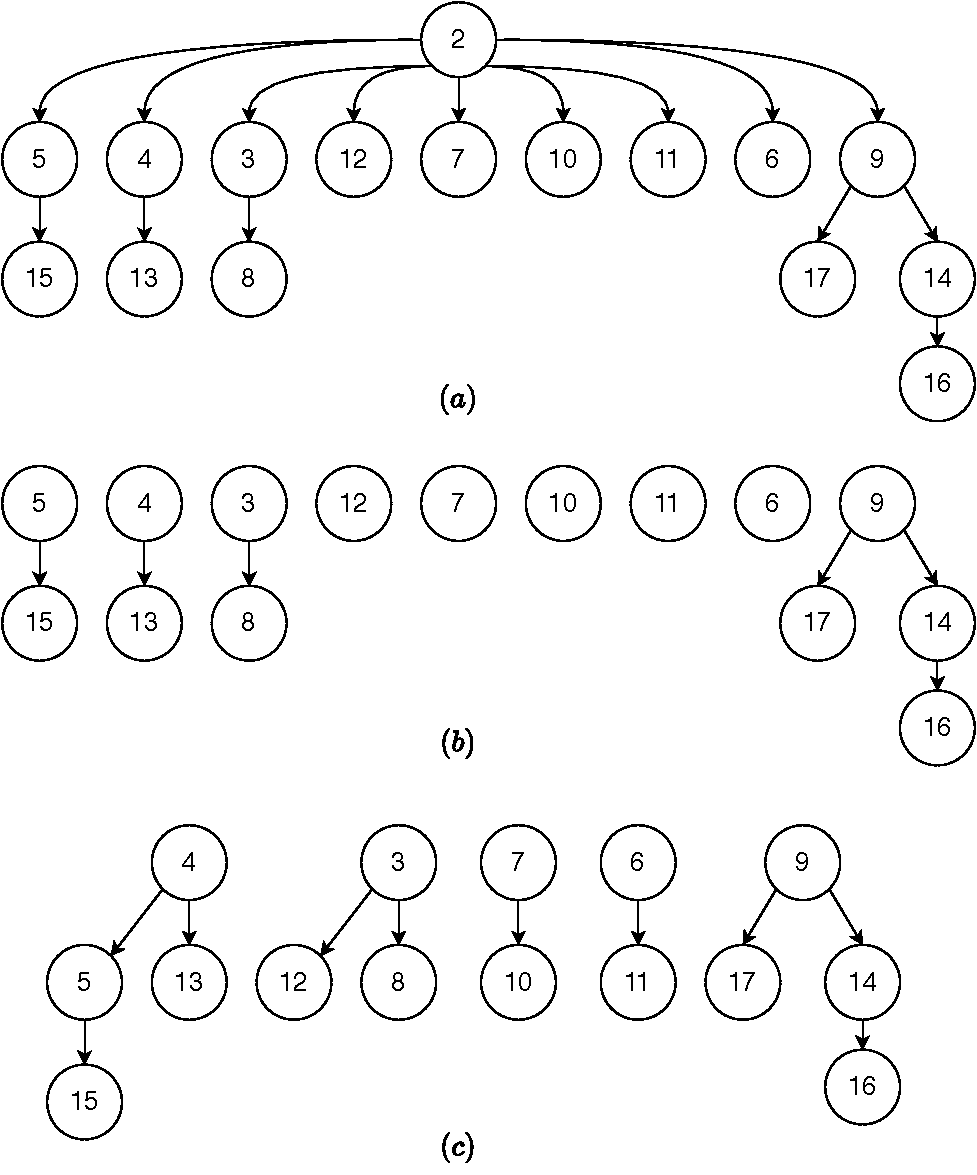
\includegraphics[scale=0.4]{img/pairs-merge}} \\
  \caption{删除根节点,将子树成对合并}
  \label{fig:merge-pairs}
\end{figure}

\begin{figure}[htbp]
  \centering
  \subcaptionbox{将根节点为9和6的两棵树合并}{\hspace{0.2\textwidth}\includegraphics[scale=0.4]{img/right-merge-1}\hspace{0.2\textwidth}}
  \subcaptionbox{将根节点为7的树合并到当前结果中}{\hspace{0.1\textwidth}\includegraphics[scale=0.4]{img/right-merge-2}\hspace{0.1\textwidth}} \\
  \subcaptionbox{将根节点为3的树合并到结果中}{\hspace{0.1\textwidth}\includegraphics[scale=0.4]{img/right-merge-3}\hspace{0.1\textwidth}}
  \subcaptionbox{将根节点为4的树合并到结果中}{\hspace{0.1\textwidth}\includegraphics[scale=0.4]{img/right-merge-4}\hspace{0.1\textwidth}}
  \caption{从右向左合并的步骤}
  \label{fig:merge-right}
\end{figure}

\be
\begin{array}{rcl}
\textit{consolidate}\ [\ ] & = & \nil \\
\textit{consolidate}\ [t] & = & t \\
\textit{consolidate}\ (t_1 : t_2 : ts) & = & merge\ (merge\ t_1\ t_2)\ (consolidate\ ts)
\end{array}
\ee

对应“左侧孩子,右侧兄弟”的实现如下:

\begin{algorithmic}[1]
\Function{Pop}{$H$}
  \State $L \gets$ NIL
  \For{every $T_x$, $T_y$ in \Call{Sub-Trees}{$H$}}
    \State $T \gets $ \Call{Merge}{$T_x, T_y$}
    \State $L \gets$ \Call{Link}{$T, L$}
  \EndFor
  \State $H \gets$ NIL
  \For{$T$ in $L$}
    \State $H \gets $ \Call{Merge}{$H, T$}
  \EndFor
  \State \Return $H$
\EndFunction
\end{algorithmic}

我们从左向右每次成对迭代两棵子树$T_x$、$T_y$合并成$T$,然后链接到$L$的前面。这样再次遍历$L$时,实际是按照从右向左的顺序。堆中可能含有奇数棵子树,这种情况下,最后一次$T_y =$ NIL,成对合并后$T = T_x$。

\subsection{删除}
\index{配对堆!删除}

为了删除某个节点$x$,我们可以先将节点的值减小为$-\infty$,然后再执行一次弹出操作。本节介绍另外一种删除方法。若$x$为根节点,我们只需要执行一次弹出操作。否则,我们将$x$从堆$H$中切下,然后对$x$执行一次弹出操作,再将结果合并回$H$:

\begin{algorithmic}[1]
\Function{Delete}{$H, x$}
  \If{$H = x$}
    \State \Call{Pop}{$H$}
  \Else
    \State $H \gets$ \Call{Cut}{$H, x$}
    \State $x \gets$ \Call{Pop}{$x$}
    \State \Call{Merge}{$H, x$}
  \EndIf
\EndFunction
\end{algorithmic}

因为删除算法调用弹出操作,我们猜想它的分摊性能也是对数时间$O(\lg n)$。

\begin{Exercise}
实现配对堆的删除。
\end{Exercise}

\section{小结}

本章中,我们将堆的实现从二叉树扩展到了更加丰富的数据结构。二项式堆和斐波那契堆使用多叉树森林作为底层数据结构,而配对堆实现为一棵多叉树。通过将某些耗时的操作延迟进行,可以获得总体上优异的分摊性能。这一点很具有启发性。

\section{附录:例子程序}

多叉树的定义(左侧孩子,右侧兄弟):

\begin{lstlisting}[language = Bourbaki]
data Node<K> {
    Int rank
    K key
    Node<K> parent, subTrees, sibling,
    Bool mark

    Node(K x) {
        key = x
        rank = 0
        parent = subTrees = sibling = null
        mark = false
    }
}
\end{lstlisting}

二项式树链接:

\begin{lstlisting}[language = Bourbaki]
Node<K> link(Node<K> t1, Node<K> t2) {
    if t2.key < t1.key then (t1, t2) = (t2, t1)
    t2.sibling = t1.subTrees
    t1.subTrees = t2
    t2.parent = t1
    t1.rank = t1.rank + 1
    return t1
}
\end{lstlisting}

二项式堆插入:

\begin{lstlisting}[language = Bourbaki]
Node<K> insert(K x, Node<K> h) = insertTree(Node(x), h)

Node<K> insertTree(Node<K> t, Node<K> h) {
    var h1 = Node()
    var prev = h1
    while h != null and h.rank <= t.rank {
        var t1 = h
        h = h.sibling
        if t.rank == t1.rank {
            t = link(t, t1)
        } else {
            prev.sibling = t1
            prev = t1
        }
    }
    prev.sibling = t
    t.sibling = h
    return removeFirst(h1)
}

Node<K> removeFirst(Node<K> h) {
    var next = h.sibling
    h.sibling = null
    return next
}
\end{lstlisting}

二项式堆插入的递归实现:

\begin{Haskell}
data BiTree a = Node { rank :: Int
                     , key :: a
                     , subTrees :: [BiTree a]}

type BiHeap a = [BiTree a]

link t1@(Node r x c1) t2@(Node _ y c2) =
    if x < y then Node (r + 1) x (t2:c1)
    else Node (r + 1) y (t1:c2)

insertTree t [] = [t]
insertTree t ts@(t':ts') | rank t < rank t' = t:ts
                         | rank t > rank t' = t' : insertTree t ts'
                         | otherwise = insertTree (link t t') ts'

insert x = insertTree (Node 0 x [])
\end{Haskell}

二项式堆的合并:

\begin{lstlisting}[language = Bourbaki]
Node<K> merge(h1, h2) {
    var h = Node()
    var prev = h
    while h1 != null and h2 != null {
        if h1.rank < h2.rank {
            prev.sibling = h1
            prev = prev.sibling
            h1 = h1.sibling
        } else if h2.rank < h1.rank {
            prev.sibling = h2
            prev = prev.sibling
            h2 = h2.sibling
        } else {
            var (t1, t2) = (h1, h2)
            (h1, h2) = (h1.sibling, h2.sibling)
            h1 = insertTree(link(t1, t2), h1)
    }
    if h1 != null then prev.sibling = h1
    if h2 != null then prev.sibling = h2
    return removeFirst(h)
}
\end{lstlisting}

递归合并两个二项式堆:

\begin{Haskell}
merge ts1 [] = ts1
merge [] ts2 = ts2
merge ts1@(t1:ts1') ts2@(t2:ts2')
    | rank t1 < rank t2 = t1:(merge ts1' ts2)
    | rank t1 > rank t2 = t2:(merge ts1 ts2')
    | otherwise = insertTree (link t1 t2) (merge ts1' ts2')
\end{Haskell}

二项式堆的弹出

\begin{lstlisting}[language = Bourbaki]
Node<K> reverse(Node<K> h) {
    Node<K> prev = null
    while h != null {
        var x = h
        h = h.sibling
        x.sibling = prev
        prev = x
    }
    return prev
}

(Node<K>, Node<K>) extractMin(Node<K> h) {
    var head = h
    Node<K> tp = null
    Node<K> tm = null
    Node<K> prev = null
    while h != null {
        if tm == null or h.key < tm.key {
            tm = h
            tp = prev
        }
        prev = h
        h = h.sibling
    }
    if tp != null {
        tp.sibling = tm.sibling
    } else {
        head = tm.sibling
    }
    tm.sibling = null
    return (tm, head)
}

(K, Node<K>) pop(Node<K> h) {
    var (tm, h) = extractMin(h)
    h = merge(h, reverse(tm.subtrees))
    tm.subtrees = null
    return (tm.key, h)
}
\end{lstlisting}

二项式堆弹出的递归实现:

\begin{Haskell}
pop h = merge (reverse $ subTrees t) ts where
    (t, ts) = extractMin h

extractMin [t] = (t, [])
extractMin (t:ts) = if key t < key t' then (t, ts)
                    else (t', t:ts') where
    (t', ts') = extractMin ts
\end{Haskell}

使用双向链表合并斐波那契堆:

\begin{lstlisting}[language = Bourbaki]
FibHeap<K> merge(FibHeap<K> h1, FibHeap<K> h2) {
    if isEmpty(h1) then return h2
    if isEmpty(h2) then return h1
    FibHeap<K> h = FibHeap<K>()
    h.trees = concat(h1.trees, h2.trees)
    h.minTree = if h1.minTree.key < h2.minTree.key
                then h1.minTree else h2.minTree
    h.size = h1.size + h2.size
    return h
}

bool isEmpty(FibHeap<K> h) = (h == null or h.trees == null)

Node<K> concat(Node<K> first1, Node<K> first2) {
  var last1 = first1.prev
  var last2 = first2.prev
  last1.next = first2
  first2.prev = last1
  last2.next = first1
  first1.prev = last2
  return first1
}
\end{lstlisting}

斐波那契树归并:

\begin{Haskell}
consolidate = foldr melt [] where
    melt t [] = [t]
    meld t (t':ts) | rank t == rank t' = meld (link t t') ts
                   | rank t <  rank t' = t : t' : ts
                   | otherwise = t' : meld t ts
\end{Haskell}

使用辅助数组进行归并:

\begin{lstlisting}[language = Bourbaki]
void consolidate(FibHeap<K> h) {
    Int R = maxRank(h.size) + 1
    Node<K>[R] a = [null, ...]
    while h.trees != null {
        var x = h.trees
        h.trees = remove(h.trees, x)
        Int r = x.rank
        while a[r] != null {
            var y = a[r]
            x = link(x, y)
            a[r] = null
            r = r + 1
        }
        a[r] = x
    }
    h.minTr = null
    h.trees = null
    for var t in a if t != null {
        h.trees = append(h.trees, t)
        if h.minTr == null or t.key < h.minTr.key then h.minTr = t
    }
}
\end{lstlisting}

斐波那契堆的弹出:

\begin{Haskell}
pop (FH _ (Node _ x []) []) = (x, E)
pop (FH sz (Node _ x tsm) ts) = (x, FH (sz - 1) tm ts') where
    (tm, ts') = extractMin $ consolidate (tsm ++ ts)
\end{Haskell} %$

提升优先级:

\begin{lstlisting}[language = Bourbaki]
void decrease(FibHeap<K> h, Node<K> x, K k) {
    var p = x.parent
    x.key = k
    if p != null and k < p.key {
        cut(h, x)
        cascadeCut(h, p)
    }
    if k < h.minTr.key then h.minTr = x
}

void cut(FibHeap<K> h, Node<K> x) {
    var p = x.parent
    p.subTrees = remove(p.subTrees, x)
    p.rank = p.rank - 1
    h.trees = append(h.trees, x)
    x.parent = null
    x.mark = false
}

void cascadeCut(FibHeap<K> h, Node<K> x) {
    var p = x.parent
    if p == null then return
    if x.mark {
        cut(h, x)
        cascadeCut(h, p)
    } else {
        x.mark = true
    }
}
\end{lstlisting}

\ifx\wholebook\relax \else
\section{参考答案}
\shipoutAnswer

\begin{thebibliography}{99}

\bibitem{K-ary-tree}
K-ary tree, Wikipedia. \url{https://en.wikipedia.org/wiki/K-ary_tree}

\bibitem{CLRS}
Thomas H. Cormen, Charles E. Leiserson, Ronald L. Rivest and Clifford Stein. ``Introduction to Algorithms, Second Edition''. The MIT Press, 2001. ISBN: 0262032937. (《算法导论》中文版)

\bibitem{okasaki-book}
Chris Okasaki. ``Purely Functional Data Structures''. Cambridge university press, (July 1, 1999), ISBN-13: 978-0521663502

\bibitem{wiki-pascal-triangle}
Wikipedia, ``Pascal's triangle''. \url{https://en.wikipedia.org/wiki/Pascal's_triangle}

\bibitem{hackage-fibq}
Hackage. ``An alternate implementation of a priority queue based on a Fibonacci heap.'', \url{http://hackage.haskell.org/packages/archive/pqueue-mtl/1.0.7/doc/html/src/Data-Queue-FibQueue.html}

\bibitem{okasaki-fibh}
Chris Okasaki. ``Fibonacci Heaps.'' \url{http://darcs.haskell.org/nofib/gc/fibheaps/orig}

\bibitem{pairing-heap}
Michael L. Fredman, Robert Sedgewick, Daniel D. Sleator, and Robert E. Tarjan. ``The Pairing Heap: A New Form of Self-Adjusting Heap'' Algorithmica (1986) 1: 111-129.

\end{thebibliography}

\expandafter\enddocument
\fi
